\section{O Futuro: Edge AI}

\begin{frame}{Inteligência Artificial de Borda (Edge AI)}
    \begin{columns}
        % --- COLUNA DA ESQUERDA (TEXTO) ---
        \begin{column}{0.55\textwidth}
            \begin{itemize}
                \item O futuro das RSSF transforma os nós sensores, antes coletores passivos, em unidades de processamento inteligente.  
                \item O \textit{Edge Computing} move a análise para a periferia da rede, eliminando a total dependência da nuvem.  
                \item Isso é viabilizado pelo \textbf{TinyML}, que roda modelos de redes neurais diretamente nos microcontroladores.  
            \end{itemize}
            
            \vspace{0.2cm}
            
            \begin{block}{A Vantagem Energética}
                O nó processa dados localmente e transmite via rádio \textbf{apenas a inferência} (resultado), economizando drasticamente a bateria.  
            \end{block}
        \end{column}
        
        % --- COLUNA DA DIREITA (IMAGEM) ---
        \begin{column}{0.45\textwidth}
            \begin{figure}
                \centering
                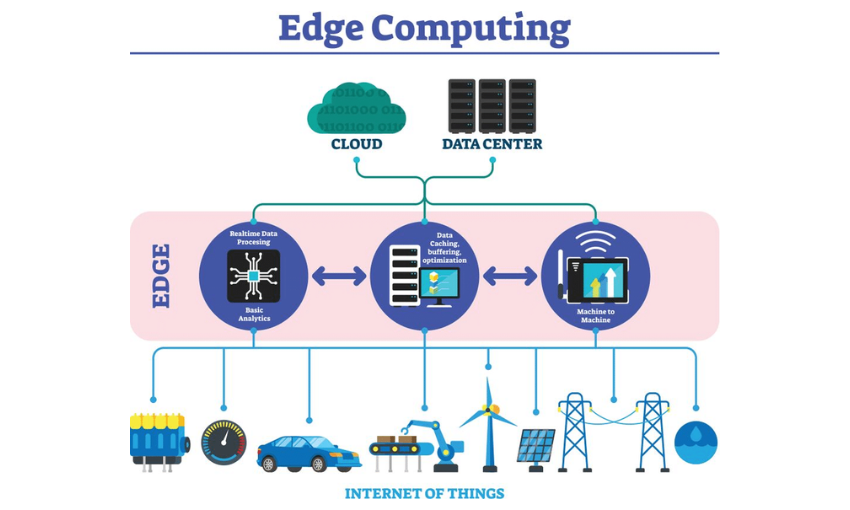
\includegraphics[width=\textwidth]{figuras/edge.png}
                \caption{A camada de Edge Computing.}
                \vspace{0.1cm}
                {\tiny Fonte: Portal Embarcados}
            \end{figure}
        \end{column}
    \end{columns}
\end{frame}

\begin{frame}{Impactos Diretos na Indústria 4.0}
    \begin{columns}
        \begin{column}{0.5\textwidth}
            \begin{itemize}
                \item A integração entre IoT e IA fornece os dados processados necessários para alimentar \textbf{Gêmeos Digitais} (\textit{Digital Twins}).  
                \item As indústrias conseguem simular o comportamento físico de seus equipamentos e prever falhas com precisão cirúrgica.  
                \item Os nós atuam como o sistema nervoso das fábricas, transformando a rede em um sistema de tomada de decisão proativo.  
            \end{itemize}
        \end{column}
        
        \begin{column}{0.5\textwidth}
            \begin{center}
                \textbf{Projeção de Impacto Econômico}\vspace{0.4cm}
                
                % --- INFOGRÁFICO FEITO EM LATEX (TIKZ) ---
                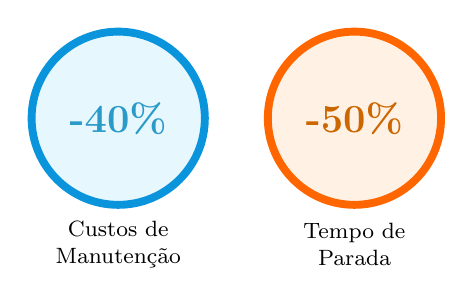
\begin{tikzpicture}
                    % Círculo 1: Manutenção (-40%)
                    \fill[cyan!10] (0,0) circle (1.1);
                    \draw[cyan!80!blue, line width=1mm] (0,0) circle (1.1);
                    \node[cyan!80!black, font=\Large\bfseries] at (0,0) {-40\%};
                    \node[align=center, font=\footnotesize] at (0,-1.6) {Custos de\\Manutenção};
                    
                    % Círculo 2: Downtime (-50%)
                    \fill[orange!10] (3,0) circle (1.1);
                    \draw[orange!80!red, line width=1mm] (3,0) circle (1.1);
                    \node[orange!80!black, font=\Large\bfseries] at (3,0) {-50\%};
                    \node[align=center, font=\footnotesize] at (3,-1.6) {Tempo de\\Parada};
                \end{tikzpicture}
                
                \vspace{0.6cm}
                {\tiny \textit{Fonte: McKinsey \& Company (Digital Manufacturing)}}
            \end{center}
        \end{column}
    \end{columns}
\end{frame}